\documentclass[3pt]{standalone}
\usepackage{tikz}
%\usepackage{tkz-graph}
%\usepackage{tikz-network}


\begin{document}

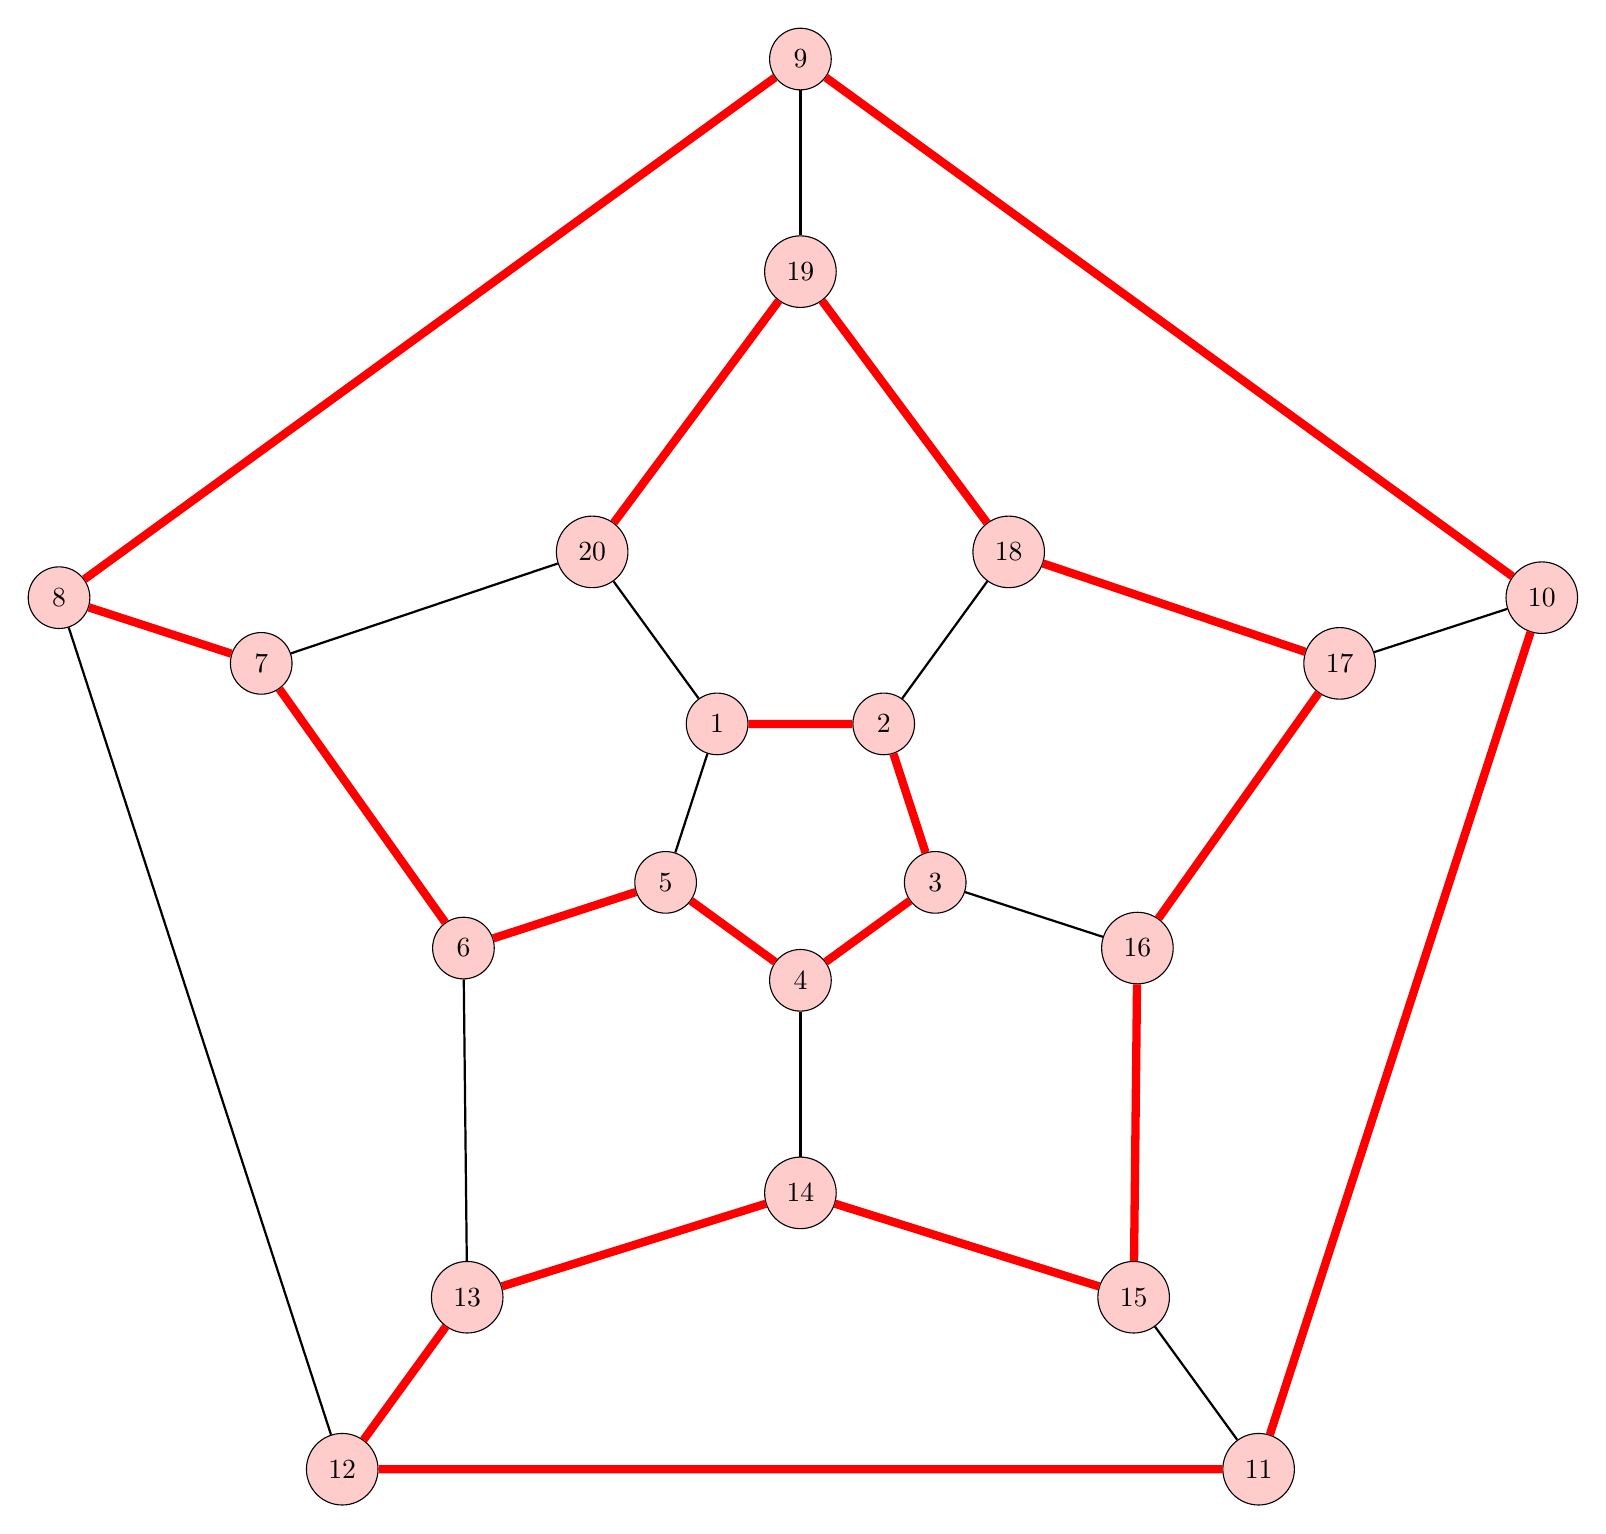
\begin{tikzpicture}[scale=0.9, inner sep=5pt, place/.style={circle,draw,fill=red!20}]
\foreach \angle/\i in {54/2,126/1,198/5,270/4,342/3}
{ 
\draw (\angle:2) node[place](\i) {$\i$};
}

\foreach \angle/\i in {54/18,126/20,198/6,270/14,342/16}
{ 
\draw (\angle:5) node[place](\i) {$\i$};
}

\foreach \angle/\i in {18/17,90/19,162/7,234/13,306/15}
{ 
\draw (\angle:8) node[place](\i) {$\i$};
}

\foreach \angle/\i in {18/10,90/9,162/8,234/12,306/11}
{ 
\draw (\angle:11) node[place](\i) {$\i$};
}

\draw[line width=3pt,red] (1) --(2) -- (3) -- (4) -- (5) -- (6) -- (7) -- (8) -- (9) -- (10) -- (11) -- (12) -- (13)-- (14) -- (15) -- (16) -- (17) -- (18) -- (19) -- (20);

\draw[thick] (5)--(1)--(20)--(7);
\draw[thick] (19)--(9);
\draw[thick] (2)--(18);
\draw[thick] (17)--(10);
\draw[thick] (3)--(16);
\draw[thick] (15)--(11);
\draw[thick] (4)--(14);
\draw[thick] (8)--(12);
\draw[thick] (6)--(13);
\end{tikzpicture}


\end{document}